\chapter{Chapter XII}

\begin{verse}
The heralds left their pricking up and down,\\
Now ringen trumpets loud and clarion.\\
There is no more to say, but east and west,\\
In go the speares sadly in the rest,\\
In goth the sharp spur into the side,\\
There see men who can just and who can ride;\\
There shiver shaftes upon shieldes thick,\\
He feeleth through the heart-spone the prick;\\
Up springen speares, twenty feet in height,\\
Out go the swordes to the silver bright;\\
The helms they to-hewn and to-shred;\\
Out burst the blood with stern streames red.\\!
\attrib{Chaucer.}
\end{verse}

\lettrine{M}{orning} arose in unclouded splendour, and ere the sun was
much above the
horizon, the idlest or the most eager of the spectators appeared on the
common, moving to the lists as to a general centre, in order to secure a
favourable situation for viewing the continuation of the expected games.

The marshals and their attendants appeared next on the field, together
with the heralds, for the purpose of receiving the names of the knights
who intended to joust, with the side which each chose to espouse. This
was a necessary precaution, in order to secure equality betwixt the two
bodies who should be opposed to each other.

According to due formality, the Disinherited Knight was to be considered
as leader of the one body, while Brian de Bois-Guilbert, who had been
rated as having done second-best in the preceding day, was named first
champion of the other band. Those who had concurred in the challenge
adhered to his party of course, excepting only Ralph de Vipont, whom his
fall had rendered unfit so soon to put on his armour. There was no want
of distinguished and noble candidates to fill up the ranks on either
side.

In fact, although the general tournament, in which all knights fought at
once, was more dangerous than single encounters, they were,
nevertheless, more frequented and practised by the chivalry of the age.
Many knights, who had not sufficient confidence in their own skill to
defy a single adversary of high reputation, were, nevertheless, desirous
of displaying their valour in the general combat, where they might meet
others with whom they were more upon an equality. On the present
occasion, about fifty knights were inscribed as desirous of combating
upon each side, when the marshals declared that no more could be
admitted, to the disappointment of several who were too late in
preferring their claim to be included.

About the hour of ten o'clock, the whole plain was crowded with
horsemen, horsewomen, and foot-passengers, hastening to the tournament;
and shortly after, a grand flourish of trumpets announced Prince John
and his retinue, attended by many of those knights who meant to take
share in the game, as well as others who had no such intention.

About the same time arrived Cedric the Saxon, with the Lady Rowena,
unattended, however, by Athelstane. This Saxon lord had arrayed his tall
and strong person in armour, in order to take his place among the
combatants; and, considerably to the surprise of Cedric, had chosen to
enlist himself on the part of the Knight Templar. The Saxon, indeed, had
remonstrated strongly with his friend upon the injudicious choice he had
made of his party; but he had only received that sort of answer usually
given by those who are more obstinate in following their own course,
than strong in justifying it.

His best, if not his only reason, for adhering to the party of Brian de
Bois-Guilbert, Athelstane had the prudence to keep to himself. Though
his apathy of disposition prevented his taking any means to recommend
himself to the Lady Rowena, he was, nevertheless, by no means insensible
to her charms, and considered his union with her as a matter already
fixed beyond doubt, by the assent of Cedric and her other friends. It
had therefore been with smothered displeasure that the proud though
indolent Lord of Coningsburgh beheld the victor of the preceding day
select Rowena as the object of that honour which it became his privilege
to confer. In order to punish him for a preference which seemed to
interfere with his own suit, Athelstane, confident of his strength, and
to whom his flatterers, at least, ascribed great skill in arms, had
determined not only to deprive the Disinherited Knight of his powerful
succour, but, if an opportunity should occur, to make him feel the
weight of his battle-axe.

De Bracy, and other knights attached to Prince John, in obedience to a
hint from him, had joined the party of the challengers, John being
desirous to secure, if possible, the victory to that side. On the other
hand, many other knights, both English and Norman, natives and
strangers, took part against the challengers, the more readily that the
opposite band was to be led by so distinguished a champion as the
Disinherited Knight had approved himself.

As soon as Prince John observed that the destined Queen of the day had
arrived upon the field, assuming that air of courtesy which sat well
upon him when he was pleased to exhibit it, he rode forward to meet her,
doffed his bonnet, and, alighting from his horse, assisted the Lady
Rowena from her saddle, while his followers uncovered at the same time,
and one of the most distinguished dismounted to hold her palfrey.

``It is thus,'' said Prince John, ``that we set the dutiful example of
loyalty to the Queen of Love and Beauty, and are ourselves her guide to
the throne which she must this day occupy.--Ladies,'' he said, ``attend
your Queen, as you wish in your turn to be distinguished by like
honours.''

So saying, the Prince marshalled Rowena to the seat of honour opposite
his own, while the fairest and most distinguished ladies present crowded
after her to obtain places as near as possible to their temporary
sovereign.

No sooner was Rowena seated, than a burst of music, half-drowned by the
shouts of the multitude, greeted her new dignity. Meantime, the sun
shone fierce and bright upon the polished arms of the knights of either
side, who crowded the opposite extremities of the lists, and held eager
conference together concerning the best mode of arranging their line of
battle, and supporting the conflict.

The heralds then proclaimed silence until the laws of the tourney should
be rehearsed. These were calculated in some degree to abate the dangers
of the day; a precaution the more necessary, as the conflict was to be
maintained with sharp swords and pointed lances.

The champions were therefore prohibited to thrust with the sword, and
were confined to striking. A knight, it was announced, might use a mace
or battle-axe at pleasure, but the dagger was a prohibited weapon. A
knight unhorsed might renew the fight on foot with any other on the
opposite side in the same predicament; but mounted horsemen were in that
case forbidden to assail him. When any knight could force his antagonist
to the extremity of the lists, so as to touch the palisade with his
person or arms, such opponent was obliged to yield himself vanquished,
and his armour and horse were placed at the disposal of the conqueror. A
knight thus overcome was not permitted to take farther share in the
combat. If any combatant was struck down, and unable to recover his
feet, his squire or page might enter the lists, and drag his master out
of the press; but in that case the knight was adjudged vanquished, and
his arms and horse declared forfeited. The combat was to cease as soon
as Prince John should throw down his leading staff, or truncheon;
another precaution usually taken to prevent the unnecessary effusion of
blood by the too long endurance of a sport so desperate. Any knight
breaking the rules of the tournament, or otherwise transgressing the
rules of honourable chivalry, was liable to be stript of his arms, and,
having his shield reversed to be placed in that posture astride upon the
bars of the palisade, and exposed to public derision, in punishment of
his unknightly conduct. Having announced these precautions, the heralds
concluded with an exhortation to each good knight to do his duty, and to
merit favour from the Queen of Beauty and of Love.

This proclamation having been made, the heralds withdrew to their
stations. The knights, entering at either end of the lists in long
procession, arranged themselves in a double file, precisely opposite to
each other, the leader of each party being in the centre of the foremost
rank, a post which he did not occupy until each had carefully marshalled
the ranks of his party, and stationed every one in his place.

It was a goodly, and at the same time an anxious, sight, to behold so
many gallant champions, mounted bravely, and armed richly, stand ready
prepared for an encounter so formidable, seated on their war-saddles
like so many pillars of iron, and awaiting the signal of encounter with
the same ardour as their generous steeds, which, by neighing and pawing
the ground, gave signal of their impatience.

As yet the knights held their long lances upright, their bright points
glancing to the sun, and the streamers with which they were decorated
fluttering over the plumage of the helmets. Thus they remained while the
marshals of the field surveyed their ranks with the utmost exactness,
lest either party had more or fewer than the appointed number. The tale
was found exactly complete. The marshals then withdrew from the lists,
and William de Wyvil, with a voice of thunder, pronounced the signal
words--``Laissez aller!'' The trumpets sounded as he spoke--the spears
of the champions were at once lowered and placed in the rests--the spurs
were dashed into the flanks of the horses, and the two foremost ranks of
either party rushed upon each other in full gallop, and met in the
middle of the lists with a shock, the sound of which was heard at a
mile's distance. The rear rank of each party advanced at a slower pace
to sustain the defeated, and follow up the success of the victors of
their party.

The consequences of the encounter were not instantly seen, for the dust
raised by the trampling of so many steeds darkened the air, and it was a
minute ere the anxious spectator could see the fate of the encounter.
When the fight became visible, half the knights on each side were
dismounted, some by the dexterity of their adversary's lance,--some by
the superior weight and strength of opponents, which had borne down both
horse and man,--some lay stretched on earth as if never more to
rise,--some had already gained their feet, and were closing hand to hand
with those of their antagonists who were in the same predicament,--and
several on both sides, who had received wounds by which they were
disabled, were stopping their blood by their scarfs, and endeavouring to
extricate themselves from the tumult. The mounted knights, whose lances
had been almost all broken by the fury of the encounter, were now
closely engaged with their swords, shouting their war-cries, and
exchanging buffets, as if honour and life depended on the issue of the
combat.

The tumult was presently increased by the advance of the second rank on
either side, which, acting as a reserve, now rushed on to aid their
companions. The followers of Brian de Bois-Guilbert shouted--``Ha!
Beau-seant! Beau-seant!\footnote{``Beau-seant'' was the name of the
Templars' banner,
which was half black, half white, to intimate, it is said, that they
were candid and fair towards Christians, but black and terrible towards
infidels.}

``--For the Temple--For the Temple!'' The opposite party shouted in
answer--``Desdichado! Desdichado!''--which watch-word they took from the
motto upon their leader's shield.

The champions thus encountering each other with the utmost fury, and
with alternate success, the tide of battle seemed to flow now toward the
southern, now toward the northern extremity of the lists, as the one or
the other party prevailed. Meantime the clang of the blows, and the
shouts of the combatants, mixed fearfully with the sound of the
trumpets, and drowned the groans of those who fell, and lay rolling
defenceless beneath the feet of the horses. The splendid armour of the
combatants was now defaced with dust and blood, and gave way at every
stroke of the sword and battle-axe. The gay plumage, shorn from the
crests, drifted upon the breeze like snow-flakes. All that was beautiful
and graceful in the martial array had disappeared, and what was now
visible was only calculated to awake terror or compassion.

Yet such is the force of habit, that not only the vulgar spectators, who
are naturally attracted by sights of horror, but even the ladies of
distinction who crowded the galleries, saw the conflict with a thrilling
interest certainly, but without a wish to withdraw their eyes from a
sight so terrible. Here and there, indeed, a fair cheek might turn pale,
or a faint scream might be heard, as a lover, a brother, or a husband,
was struck from his horse. But, in general, the ladies around encouraged
the combatants, not only by clapping their hands and waving their veils
and kerchiefs, but even by exclaiming, ``Brave lance! Good sword!'' when
any successful thrust or blow took place under their observation.

Such being the interest taken by the fair sex in this bloody game, that
of the men is the more easily understood. It showed itself in loud
acclamations upon every change of fortune, while all eyes were so
riveted on the lists, that the spectators seemed as if they themselves
had dealt and received the blows which were there so freely bestowed.
And between every pause was heard the voice of the heralds, exclaiming,
``Fight on, brave knights! Man dies, but glory lives!--Fight on--death
is better than defeat!--Fight on, brave knights!--for bright eyes behold
your deeds!''

Amid the varied fortunes of the combat, the eyes of all endeavoured to
discover the leaders of each band, who, mingling in the thick of the
fight, encouraged their companions both by voice and example. Both
displayed great feats of gallantry, nor did either Bois-Guilbert or the
Disinherited Knight find in the ranks opposed to them a champion who
could be termed their unquestioned match. They repeatedly endeavoured to
single out each other, spurred by mutual animosity, and aware that the
fall of either leader might be considered as decisive of victory. Such,
however, was the crowd and confusion, that, during the earlier part of
the conflict, their efforts to meet were unavailing, and they were
repeatedly separated by the eagerness of their followers, each of whom
was anxious to win honour, by measuring his strength against the leader
of the opposite party.

But when the field became thin by the numbers on either side who had
yielded themselves vanquished, had been compelled to the extremity of
the lists, or been otherwise rendered incapable of continuing the
strife, the Templar and the Disinherited Knight at length encountered
hand to hand, with all the fury that mortal animosity, joined to rivalry
of honour, could inspire. Such was the address of each in parrying and
striking, that the spectators broke forth into a unanimous and
involuntary shout, expressive of their delight and admiration.

But at this moment the party of the Disinherited Knight had the worst;
the gigantic arm of Front-de-Boeuf on the one flank, and the ponderous
strength of Athelstane on the other, bearing down and dispersing those
immediately exposed to them. Finding themselves freed from their
immediate antagonists, it seems to have occurred to both these knights
at the same instant, that they would render the most decisive advantage
to their party, by aiding the Templar in his contest with his rival.
Turning their horses, therefore, at the same moment, the Norman spurred
against the Disinherited Knight on the one side, and the Saxon on the
other. It was utterly impossible that the object of this unequal and
unexpected assault could have sustained it, had he not been warned by a
general cry from the spectators, who could not but take interest in one
exposed to such disadvantage.

``Beware! beware! Sir Disinherited!'' was shouted so universally, that
the knight became aware of his danger; and, striking a full blow at the
Templar, he reined back his steed in the same moment, so as to escape
the charge of Athelstane and Front-de-Boeuf. These knights, therefore,
their aim being thus eluded, rushed from opposite sides betwixt the
object of their attack and the Templar, almost running their horses
against each other ere they could stop their career. Recovering their
horses however, and wheeling them round, the whole three pursued their
united purpose of bearing to the earth the Disinherited Knight.

Nothing could have saved him, except the remarkable strength and
activity of the noble horse which he had won on the preceding day.

This stood him in the more stead, as the horse of Bois-Guilbert was
wounded, and those of Front-de-Boeuf and Athelstane were both tired with
the weight of their gigantic masters, clad in complete armour, and with
the preceding exertions of the day. The masterly horsemanship of the
Disinherited Knight, and the activity of the noble animal which he
mounted, enabled him for a few minutes to keep at sword's point his
three antagonists, turning and wheeling with the agility of a hawk upon
the wing, keeping his enemies as far separate as he could, and rushing
now against the one, now against the other, dealing sweeping blows with
his sword, without waiting to receive those which were aimed at him in
return.

But although the lists rang with the applauses of his dexterity, it was
evident that he must at last be overpowered; and the nobles around
Prince John implored him with one voice to throw down his warder, and to
save so brave a knight from the disgrace of being overcome by odds.

``Not I, by the light of Heaven!'' answered Prince John; ``this same
springald, who conceals his name, and despises our proffered
hospitality, hath already gained one prize, and may now afford to let
others have their turn.'' As he spoke thus, an unexpected incident
changed the fortune of the day.

There was among the ranks of the Disinherited Knight a champion in black
armour, mounted on a black horse, large of size, tall, and to all
appearance powerful and strong, like the rider by whom he was mounted.
This knight, who bore on his shield no device of any kind, had hitherto
evinced very little interest in the event of the fight, beating off with
seeming ease those combatants who attacked him, but neither pursuing his
advantages, nor himself assailing any one. In short, he had hitherto
acted the part rather of a spectator than of a party in the tournament,
a circumstance which procured him among the spectators the name of ``Le
Noir Faineant'', or the Black Sluggard.

At once this knight seemed to throw aside his apathy, when he discovered
the leader of his party so hard bestead; for, setting spurs to his
horse, which was quite fresh, he came to his assistance like a
thunderbolt, exclaiming, in a voice like a trumpet-call, ``Desdichado,
to the rescue!'' It was high time; for, while the Disinherited Knight
was pressing upon the Templar, Front-de-Boeuf had got nigh to him with
his uplifted sword; but ere the blow could descend, the Sable Knight
dealt a stroke on his head, which, glancing from the polished helmet,
lighted with violence scarcely abated on the ``chamfron'' of the steed,
and Front-de-Boeuf rolled on the ground, both horse and man equally
stunned by the fury of the blow. ``Le Noir Faineant'' then turned his
horse upon Athelstane of Coningsburgh; and his own sword having been
broken in his encounter with Front-de-Boeuf, he wrenched from the hand
of the bulky Saxon the battle-axe which he wielded, and, like one
familiar with the use of the weapon, bestowed him such a blow upon the
crest, that Athelstane also lay senseless on the field. Having achieved
this double feat, for which he was the more highly applauded that it was
totally unexpected from him, the knight seemed to resume the
sluggishness of his character, returning calmly to the northern
extremity of the lists, leaving his leader to cope as he best could with
Brian de Bois-Guilbert. This was no longer matter of so much difficulty
as formerly. The Templars horse had bled much, and gave way under the
shock of the Disinherited Knight's charge. Brian de Bois-Guilbert rolled
on the field, encumbered with the stirrup, from which he was unable to
draw his foot. His antagonist sprung from horseback, waved his fatal
sword over the head of his adversary, and commanded him to yield
himself; when Prince John, more moved by the Templars dangerous
situation than he had been by that of his rival, saved him the
mortification of confessing himself vanquished, by casting down his
warder, and putting an end to the conflict.

It was, indeed, only the relics and embers of the fight which continued
to burn; for of the few knights who still continued in the lists, the
greater part had, by tacit consent, forborne the conflict for some time,
leaving it to be determined by the strife of the leaders.

The squires, who had found it a matter of danger and difficulty to
attend their masters during the engagement, now thronged into the lists
to pay their dutiful attendance to the wounded, who were removed with
the utmost care and attention to the neighbouring pavilions, or to the
quarters prepared for them in the adjoining village.

Thus ended the memorable field of Ashby-de-la-Zouche, one of the most
gallantly contested tournaments of that age; for although only four
knights, including one who was smothered by the heat of his armour, had
died upon the field, yet upwards of thirty were desperately wounded,
four or five of whom never recovered. Several more were disabled for
life; and those who escaped best carried the marks of the conflict to
the grave with them. Hence it is always mentioned in the old records, as
the Gentle and Joyous Passage of Arms of Ashby.

It being now the duty of Prince John to name the knight who had done
best, he determined that the honour of the day remained with the knight
whom the popular voice had termed ``Le Noir Faineant.'' It was pointed
out to the Prince, in impeachment of this decree, that the victory had
been in fact won by the Disinherited Knight, who, in the course of the
day, had overcome six champions with his own hand, and who had finally
unhorsed and struck down the leader of the opposite party. But Prince
John adhered to his own opinion, on the ground that the Disinherited
Knight and his party had lost the day, but for the powerful assistance
of the Knight of the Black Armour, to whom, therefore, he persisted in
awarding the prize.

To the surprise of all present, however, the knight thus preferred was
nowhere to be found. He had left the lists immediately when the conflict
ceased, and had been observed by some spectators to move down one of the
forest glades with the same slow pace and listless and indifferent
manner which had procured him the epithet of the Black Sluggard. After
he had been summoned twice by sound of trumpet, and proclamation of the
heralds, it became necessary to name another to receive the honours
which had been assigned to him. Prince John had now no further excuse
for resisting the claim of the Disinherited Knight, whom, therefore, he
named the champion of the day.

Through a field slippery with blood, and encumbered with broken armour
and the bodies of slain and wounded horses, the marshals of the lists
again conducted the victor to the foot of Prince John's throne.

``Disinherited Knight,'' said Prince John, ``since by that title only
you will consent to be known to us, we a second time award to you the
honours of this tournament, and announce to you your right to claim and
receive from the hands of the Queen of Love and Beauty, the Chaplet of
Honour which your valour has justly deserved.'' The Knight bowed low and
gracefully, but returned no answer.

While the trumpets sounded, while the heralds strained their voices in
proclaiming honour to the brave and glory to the victor--while ladies
waved their silken kerchiefs and embroidered veils, and while all ranks
joined in a clamorous shout of exultation, the marshals conducted the
Disinherited Knight across the lists to the foot of that throne of
honour which was occupied by the Lady Rowena.

On the lower step of this throne the champion was made to kneel down.
Indeed his whole action since the fight had ended, seemed rather to have
been upon the impulse of those around him than from his own free will;
and it was observed that he tottered as they guided him the second time
across the lists. Rowena, descending from her station with a graceful
and dignified step, was about to place the chaplet which she held in her
hand upon the helmet of the champion, when the marshals exclaimed with
one voice, ``It must not be thus--his head must be bare.'' The knight
muttered faintly a few words, which were lost in the hollow of his
helmet, but their purport seemed to be a desire that his casque might
not be removed.

Whether from love of form, or from curiosity, the marshals paid no
attention to his expressions of reluctance, but unhelmed him by cutting
the laces of his casque, and undoing the fastening of his gorget. When
the helmet was removed, the well-formed, yet sun-burnt features of a
young man of twenty-five were seen, amidst a profusion of short fair
hair. His countenance was as pale as death, and marked in one or two
places with streaks of blood.

\begin{figure}
    \centering
    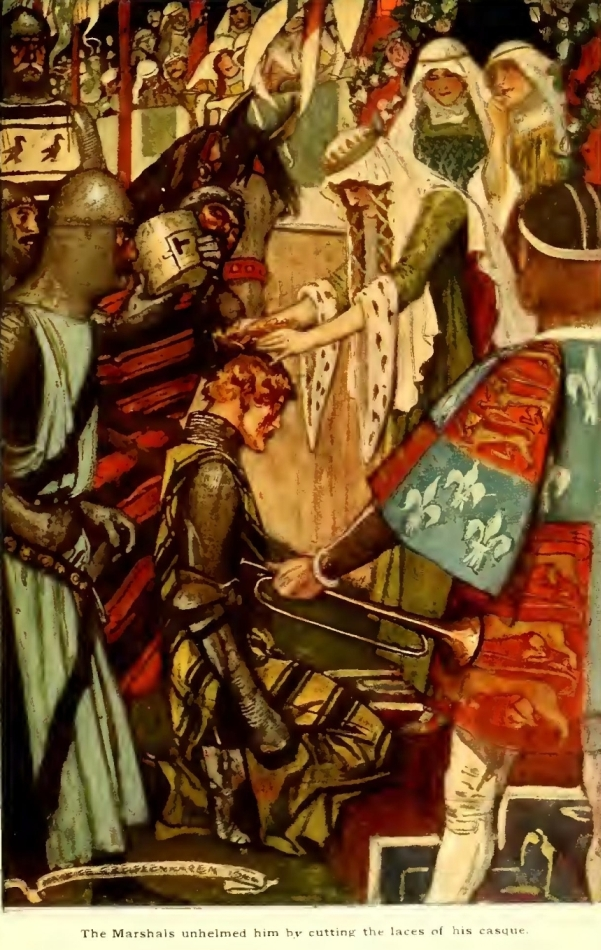
\includegraphics[height=.9\textheight]{ivanhoe/0187m}
    \caption{The Marshals unhelmed him by cutting the laces of his casque.}
\end{figure}

Rowena had no sooner beheld him than she uttered a faint shriek; but at
once summoning up the energy of her disposition, and compelling herself,
as it were, to proceed, while her frame yet trembled with the violence
of sudden emotion, she placed upon the drooping head of the victor the
splendid chaplet which was the destined reward of the day, and
pronounced, in a clear and distinct tone, these words: ``I bestow on
thee this chaplet, Sir Knight, as the meed of valour assigned to this
day's victor:'' Here she paused a moment, and then firmly added, ``And
upon brows more worthy could a wreath of chivalry never be placed!''

The knight stooped his head, and kissed the hand of the lovely Sovereign
by whom his valour had been rewarded; and then, sinking yet farther
forward, lay prostrate at her feet.

There was a general consternation. Cedric, who had been struck mute by
the sudden appearance of his banished son, now rushed forward, as if to
separate him from Rowena. But this had been already accomplished by the
marshals of the field, who, guessing the cause of Ivanhoe's swoon, had
hastened to undo his armour, and found that the head of a lance had
penetrated his breastplate, and inflicted a wound in his side.
